\section{Introduction}

Scalar active systems are those whose large-scale dynamics is well captured by a real (scalar) field, hereafter denoted $\rho$. 
As we have seen in chapter~\ref{chap_intro}, the field $\rho$ is usually referred to as the \emph{order parameter} of the theory.
While it can in general represent various quantities related to the dynamics, here it will be most of time given by the particle density.

% At equilibrium, the minimal continuous description of scalar systems with conserved order parameter is achieved via \emph{model B} (see~\cite{HohenbergRMP} for a comprehensive classification).
% Model B indeed describes a class of equilibrium systems whose dissipative dynamics is captured by a conserved field, such that $\intd{r} \, \phi(\bm r,t) = {\rm const}$, for all times $t$,  where hereafter the variables $\bm r$ and $t$ account for space and time, respectively, while $d$ denotes the number of spatial dimensions.
% As model B describes the universal large-scale features of many systems, it can be formulated based on relevant symmetries and conservation laws.
% Such a phenomenological approach can moreover be supplemented by direct coarse-graining from microscopic (particle-based) theories, which provide additional physical insights. 

% In these notes, we will apply both approaches---phenomenological and coarse-graining---to study the dynamics of scalar active systems.
% We begin with a bottom-up approach
% In \autoref{chapter: introduction}, we introduced the active Brownian particle (ABP). 
% By extending this model to a collection of interacting ABPs, we will employ coarse-graining techniques to obtain one of the paradigmatic examples of collective active matter, motility-induced phase separation (MIPS).
% Here we will review some of the essentials of equilibrium phase separation physics, what changes for methods that do not admit an equilibrium description, and discuss what is needed for this to be the case.
% We will then take a more phenomenological approach to derive the Active Model B (AMB) and the Non-Reciprocal Cahn-Hilliard (NRCH) model, and explore their rich out-of-equilibrium features.



\section{Interacting Active Brownian particles}

In Chapter~\ref{chap_intro}, we have introduced a simple model of noninteracting active Brownian particles. 
Here, we consider the simplest extension of this model by assuming that we have isotropic particles that interact via volume exclusion. 
For simplicity, we restrict our analysis to two spatial dimensions, most of what we present below will also hold in $d=3$.

We thus have $N$ active particles defined by their positions $\bm r_i$ and self-propulsion orientations $\theta_i$, $i \in \{1, \dots N\}$.
As we have seen before, we can write their dynamics in terms of overdamped Langevin equations
% The dynamics of each of these particles are described by an underdamped Langevin equation with an active velocity, as in \autoref{chapter: introduction}.
% Without interaction, it 
% %
% \begin{align}
%     \odv{\bm r_i}{t} = \bm v_{i,a}(t) + \sqrt{ 2 D_t } \bm \xi_i(t),
% \end{align}
% %
% where $\bm \xi_i(t)$ is white Gaussian noise, which obey
% %
% \begin{align}
%     \E{\xi_{k,i}(t)} &= 0, &
%     \E{\xi_{k,i}(t)\xi_{k',j}(t')} = \delta_{ij} \delta_{kk'} \delta(t - t').
% \end{align}
% %
% In two dimensions, the active velocity may be parametrized in terms of a single angle, $\bm v_a(t) = v_0 \hat {\bm e}(\theta(t))$, where 
% %
% \begin{align}
%     \hat {\bm e}(\theta) 
%     =
%     \begin{pmatrix}
%         \cos \theta \\ \sin \theta
%     \end{pmatrix}.
% \end{align}
%
%We focus on times much larger than the time scale of the rotational noise, $t\gg \tau_r = 1 / D_r$, so we may consider the rotational noise $\xi_i(t)$ to be white Gaussian noise as well.
%Including the interaction potential $U$, the full equations of motion for each particle becomes
%
\begin{subequations}
\label{eq_Langevin_int_ABPs}
\begin{align}
    \odv{\bm r_i}{t} & = v_0 \hat {\bm e}(\theta_i) - \frac{1}{\zeta} \nabla_{\bm r_i} U(\{\bm r_j\}) + \sqrt{ 2 D } \bm \xi_i, \\
    \odv{\theta_i}{t} & = \sqrt{ 2 D_r } \chi_i,
\end{align}
\end{subequations}
%
where $\zeta$ and $D$ correspond respectively to the friction and diffusivity and are related by the relation $D = k_B T / \zeta$,
while $D_r$ denotes the rotational diffusivity of the self-propulsion direction.
As before, the noises in~\eqref{eq_Langevin_int_ABPs} are Gaussian with zero mean and satisfy
\begin{equation*}
    \E{\xi_{k,i}(t)\xi_{k',j}(t')} = \delta_{kk'}\delta_{ij} \delta(t - t'), \qquad
    \E{\chi_{k}(t)\chi_{k'}(t')} = \delta_{kk'} \delta(t - t'). 
    %\qquad k,k' \in \{1,\ldots,N\}, \quad i,j \in \{1,2\}.
\end{equation*}
The interactions between the particles are modeled via a potential $U$, which we assume of the form
%
\begin{align*}
    U(\bm r_1, ..., \bm r_n) = \sum_{i \neq j} u(|\bm r_i - \bm r_j|).
\end{align*}
%
In the following, we also assume that $u$ is short-ranged, isotropic and repulsive: two particles only interact when they get in contact, while the amplitude and direction of the resulting force only depend on the vector joining their centers of mass.
The simplest choice satisfying these criteria is the hard-core potential 
\begin{equation*}
    u_{\rm HC}(r) = \begin{cases} +\infty & {\rm if}\; r < d_0\\
        0 & {\rm otherwise} \end{cases} ,
 \end{equation*}
with $d_0$ the particle diameter, 
that prevents any overlap between the particles.  
In practice --i.e. for simulations-- the hard core potential is often approximated via the Weeks-Chandler-Andersen potential (or truncated Lehnnard-Jones potential):
\begin{equation*}
    u_{\rm WCA}(r) = \begin{cases} 4\epsilon\left[ \left(\frac{d_0}{r}\right)^{12} - \left(\frac{d_0}{r}\right)^{6} \right] + \epsilon & {\rm if}\; r < 2^{1/6} d_0\\
        0 & {\rm otherwise} \end{cases} .
 \end{equation*}
Alternatively, one can also `allow' for finite overlap between particles by using a softer repulsion potential:
\begin{equation*}
    u_{\rm soft}(r) = \begin{cases} \tfrac{k}{2}(d_0 - r)^2 & {\rm if}\; r < d_0\\
        0 & {\rm otherwise} \end{cases} .
 \end{equation*}
 All the aspects that we describe below are qualitatively independent of the specific choice of the interaction potential.

\begin{figure}[!t]
    \centering
    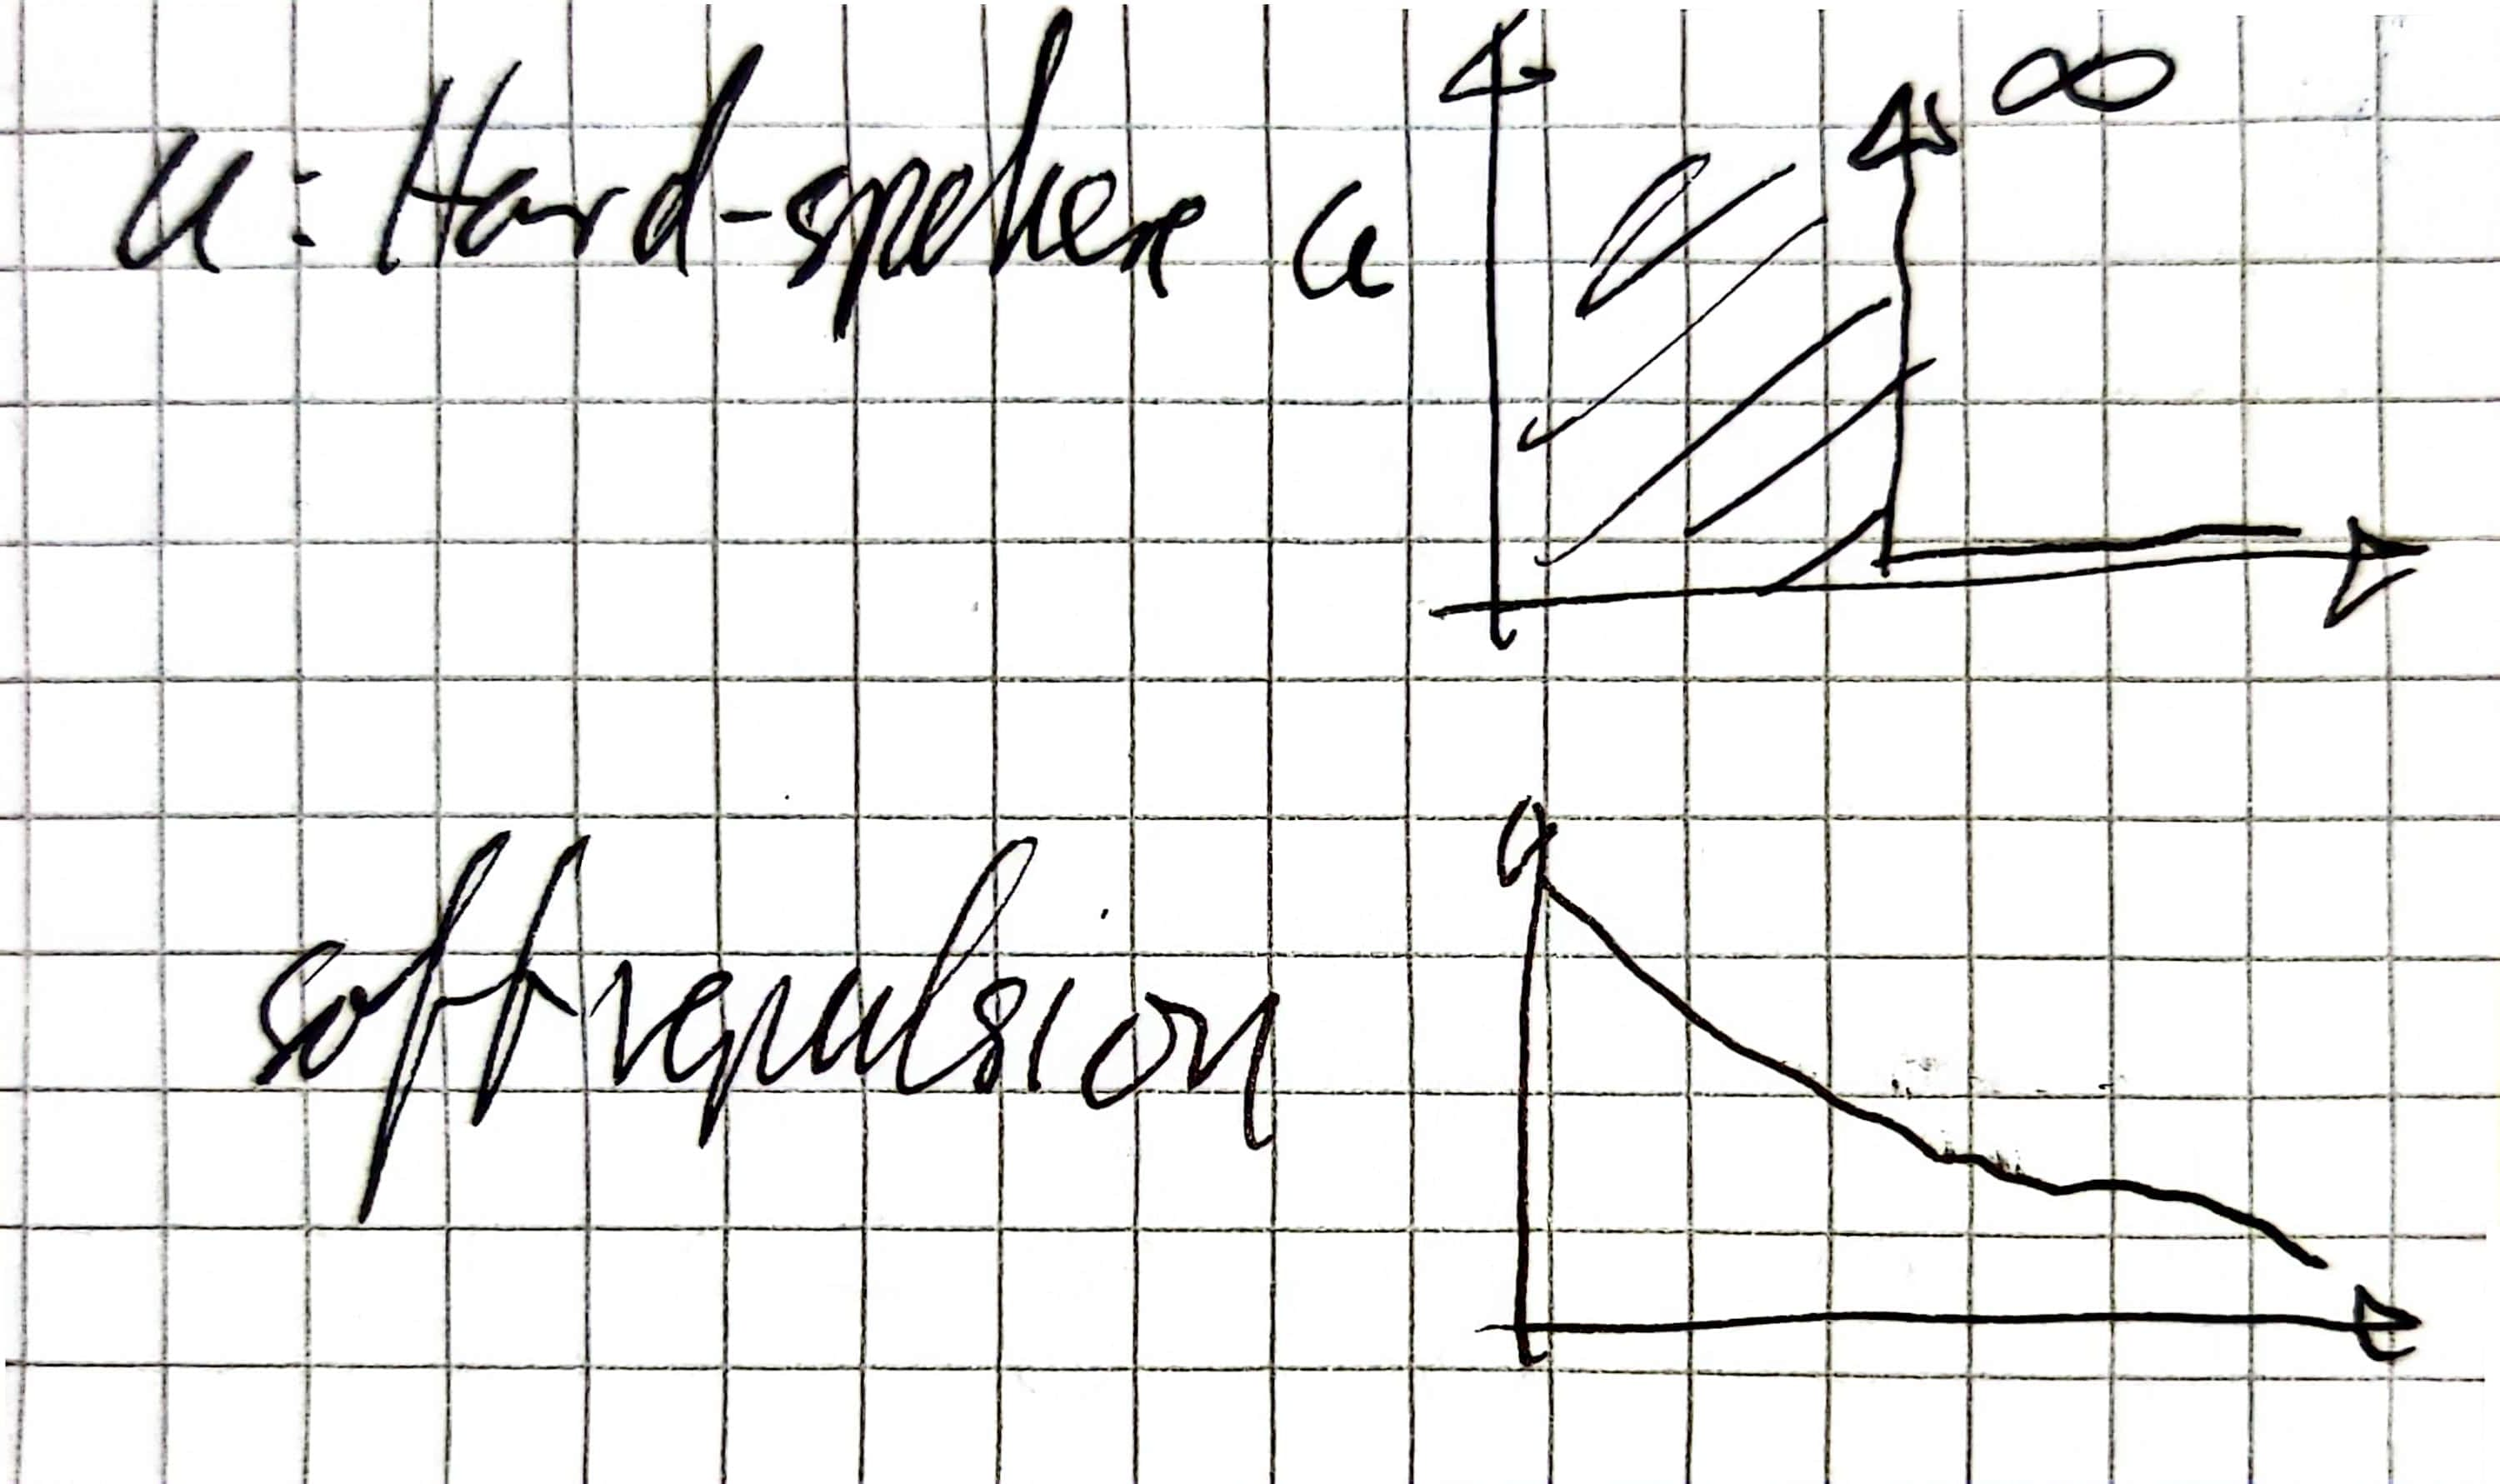
\includegraphics[width=.4\textwidth]{chapters/Figures/scalar/scalar_01.jpg}
    \caption{Illustration of the possible choices for the potential $u$. A hard repulsion corresponds to $\lim_{r\to0} u(r) = +\infty$, such that the particles can never fully overlap. On the other hand, for the soft repulsion the maximum value of the potential is finite, such that overlaps are always possible.}
    \label{fig: hard soft}
\end{figure}


In \autoref{chapter: introduction}, we wrote down the Fokker-Planck equation for the single particle, \autoref{eq_FP_BM}, which describes the time evolution of the probability distribution of the system, $\calP(\bm x, t) = \E{\delta(\bm r(t) - x)}$.
We can likewise write the Fokker-Planck for a single active Brownian particle, whose probability-density also depends on the angle of said particle
%
\begin{align}
    \calP(\bm x, \phi, t)
    =
    \E{\delta(\bm x - \bm r(t))\delta(\phi - \theta(t))}.
\end{align}
%
This obeys the Fokker-Planck equation
%
\begin{align}
    \partial_t \calP(\bm x, \phi, t)
    + \bm \nabla \cdot [
        v_0 \hat {\bm e}(\phi ) \calP(\bm r, \phi, t)
        - D \bm \nabla \calP(\bm x, \phi, t)
    ]
        - D_r \partial_\phi^2 \calP(\bm x, \phi, t)
        = 0,
\end{align}
%
which describes how the probability distribution of a single ABP, or equivalently density of a large number of non-interacting ABPs, evolves with time.

When we consider $N$ \emph{interacting} particles, however, the picture becomes significantly more complicated.
We now have to consider the $N$-body distribution,
%
\begin{align}
    \calP_N(\{\bm x_i, \phi_i\}, t) = \E{ \prod_i \delta(\bm r_i(t) - \bm x_i)\delta(\theta_i(t) - \phi_i) },
\end{align}
%
and its corresponding Fokker-Planck.
If the particles are non-interacting, the probability distribution simply factors into $N$ independent one-body distributions, while interactions introduce non-trivial correlations.
One way of tackling this is the Bogoliubov-Born-Green-Kirkwood-Yvon (BBGKY) hierarchy, which is described in \autoref{appendxi: BBKGY}.
We will instead make a simplifying mean-field assumption about the effects of the interaction.

Consider a single particle moving freely, far from any other particles.
This will move at a velocity close to the self-propulsion velocity.
If, instead, the particle is in an area with a high density, the other particles will act as barriers due to their repulsive interactions, slowing our particle down.
As an analogy, imagine the difference between running in an open feel versus trying to move in a crowd at a concert.
With this picture in mind, we assume that the effective self-propulsion speed will be lowered as the local density of particles increases, and replace the constant self-propulsion speed with one that depends on the density $\rho$,
%
\begin{align}
    v_0 &\rightarrow v(\rho), &
    \odv{v}{\rho} & < 0,
\end{align}
%
and neglect any other effects of the interaction between the particles.
The Fokker-Planck equation for the one-particle density is then
%
\begin{align} \label{eq: mips fokker planck}
    \partial_t \calP(\bm r, \phi, t)
    + \bm \nabla \cdot [
        v(\rho) \hat {\bm e}(\phi ) \calP(\bm r, \phi, t)
        - D \bm \nabla \calP(\bm r, \phi, t)
    ]
        - D_r \partial_\phi^2 \calP(\bm r, \phi, t)
        = 0,
\end{align}
%
This equation has no simple analytical solution.
However, in the regime where $t\gg 1 / D_R \equiv \tau_R$ it may be described well using \emph{moment expansion}.
This is a powerful technique is is also very useful for more complex situations.


\subsection{Spatial variation}

Before we start with the momentum expansion, we consider the case where the local velocity depends on space directly, not through the density of particles.
This can be achieved experimentally by engineering the environment of active particles, which leads to rich behavior.\todo{add sources, discuss more?}
The Fokker-Planck is then
%
\begin{align} \label{eq: mips fokker planck}
    \partial_t \calP(\bm x, \phi, t)
    + \bm \nabla \cdot [
        v(\bm x) \hat {\bm e}(\phi ) \calP(\bm x, \phi, t)
        - D \bm \nabla \calP(\bm x, \phi, t)
    ]
        - D_r \partial_\phi^2 \calP(\bm x, \phi, t)
        = 0.
\end{align}
%
A steady state configuration $P_{SS}$ obeys by assumption $\partial_t P_{SS} = 0$.
Assuming it is isotropic, so $\partial_\phi P_{SS} = 0$, and that diffusion $D$ is small compared to the active velocity, then the steady-state distribution obeys \todo[noinline]{Are these the right assumptions?}
%
\begin{align}
    \bm \nabla \cdot [v(\bm x) \hat {\bm e}(\phi ) \calP(\bm x, \phi, t)] = 0
    \implies 
    \calP(\bm x, \phi, t) \propto \frac{1}{v(\bm x)}.
\end{align}
%
The particles thus clump together where the active velocity is high, leading to higher density, while in the regions with high active velocity, the density is low.

\begin{figure}[!htb]
    \centering
    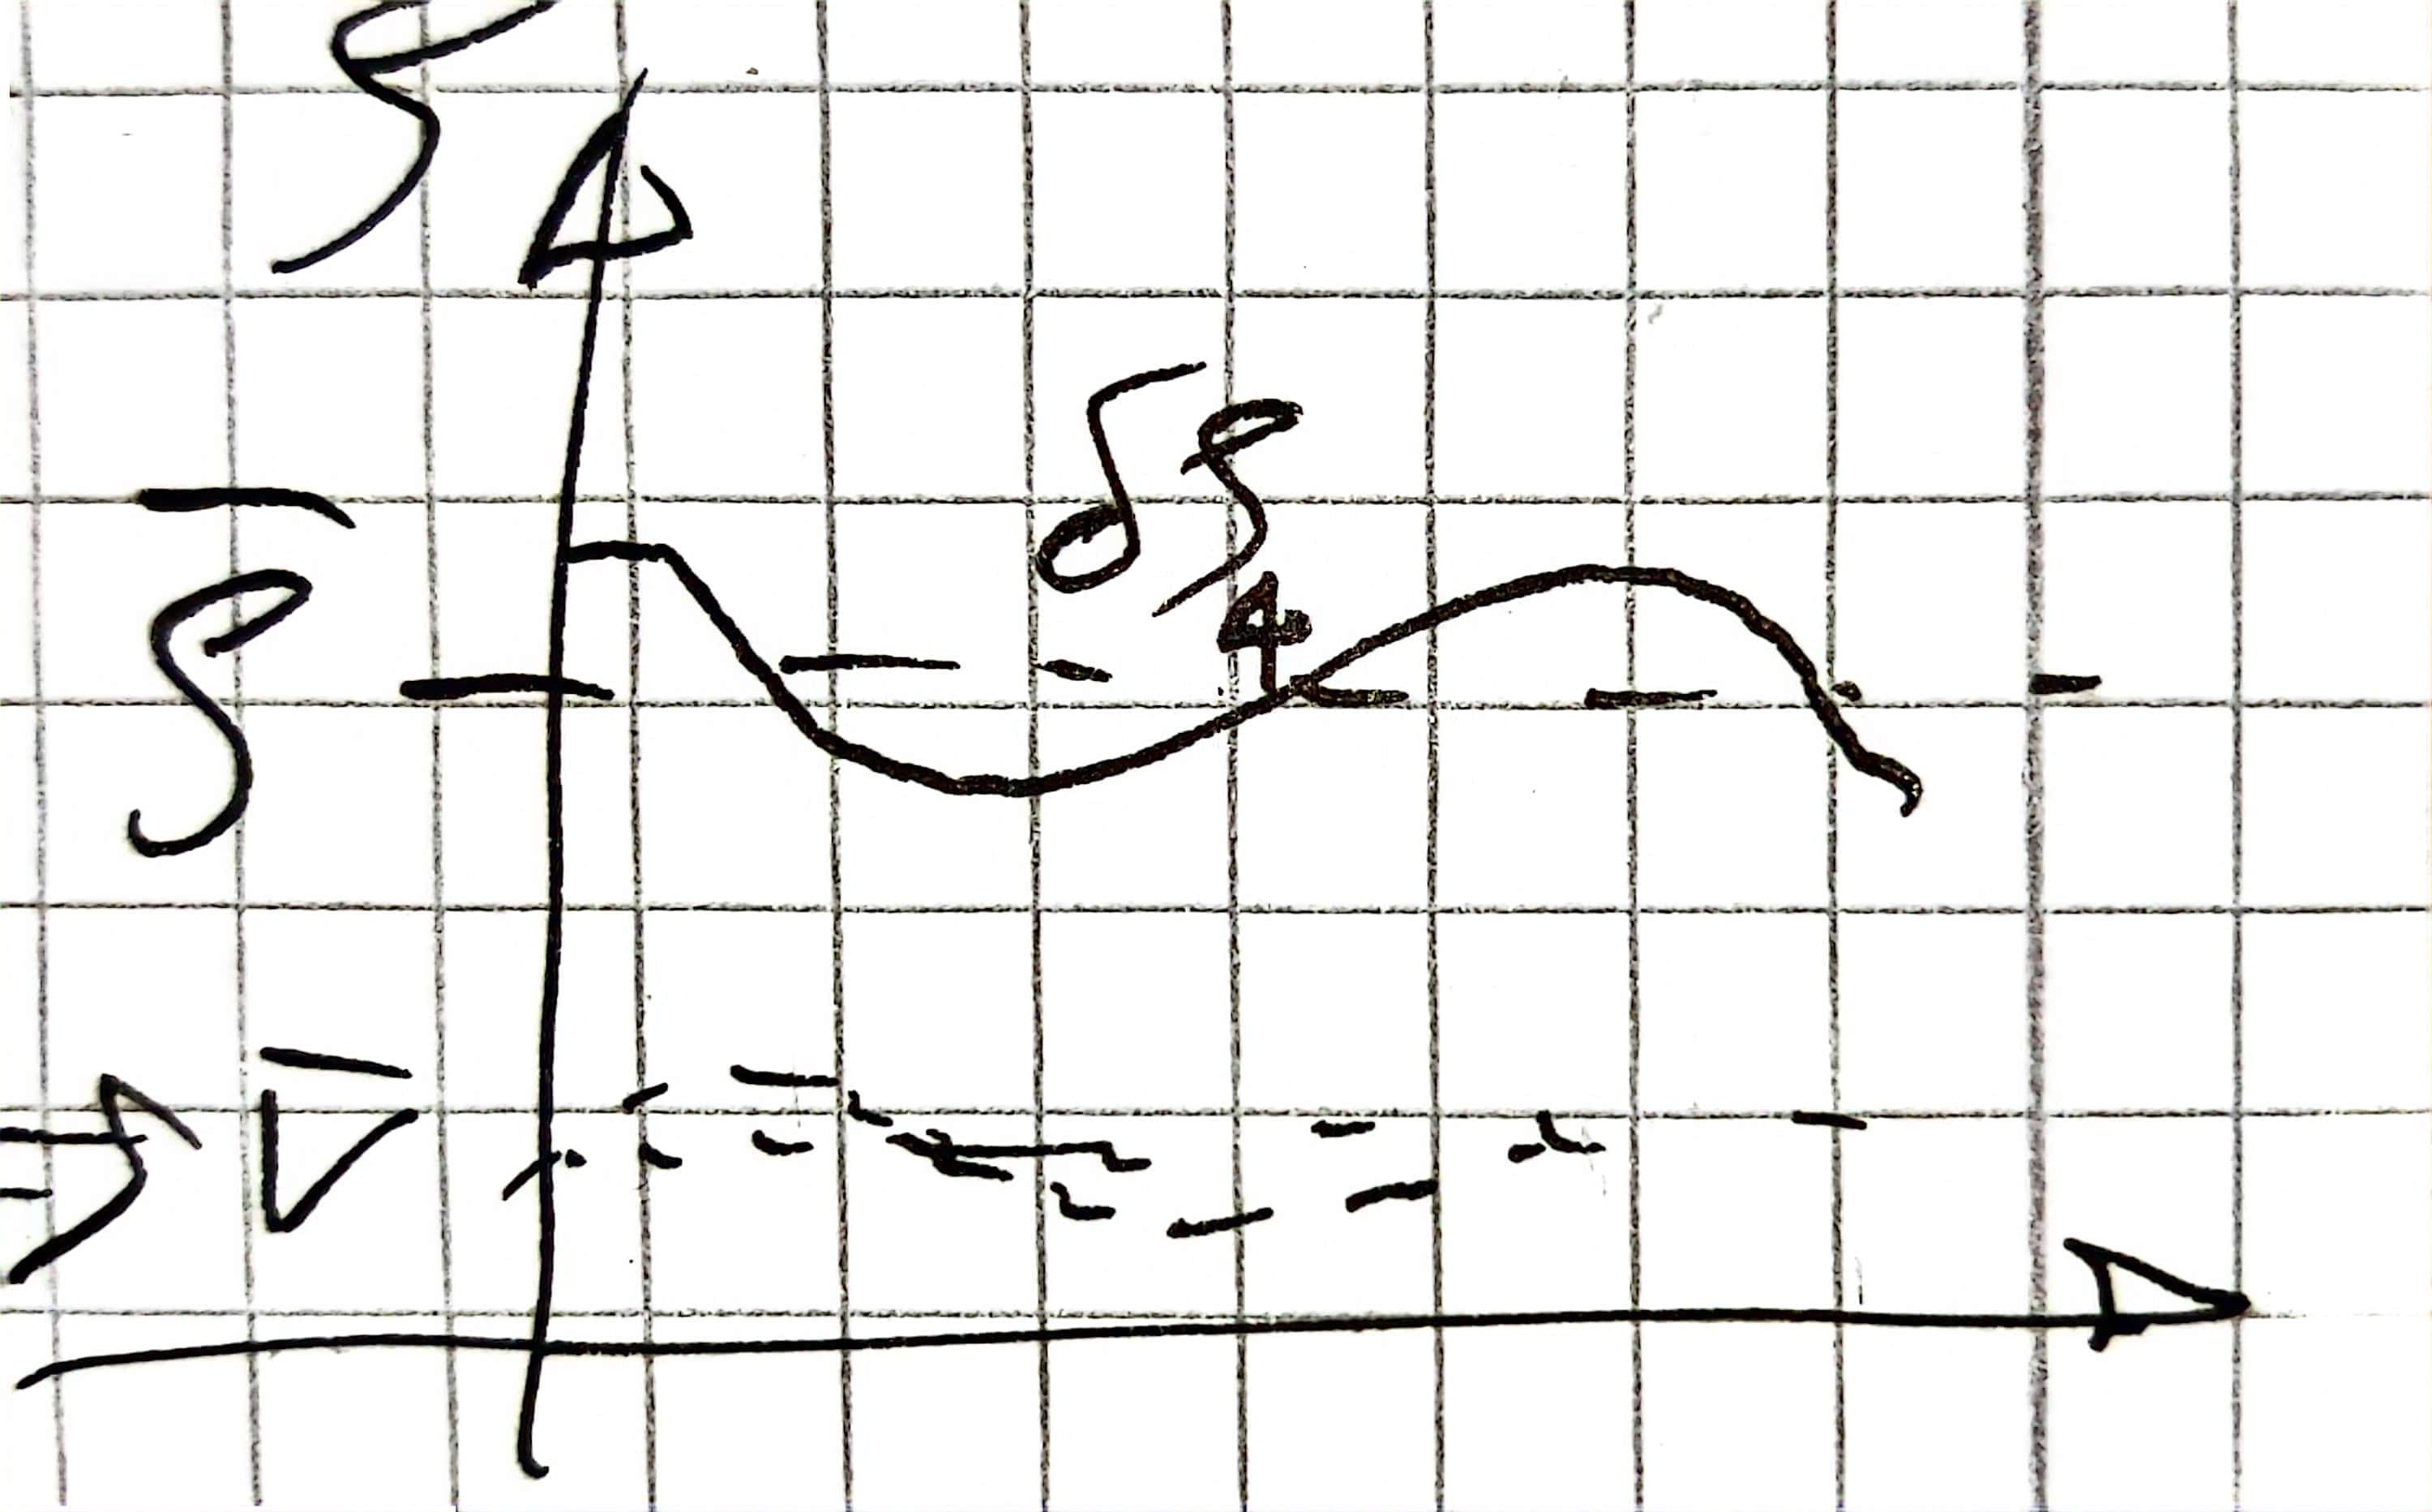
\includegraphics[width=.4\textwidth]{chapters/Figures/scalar/scalar_02.jpg}
    \caption{Perturbation in density gives perturbation in velocity}
    \label{fig: perturb}
\end{figure}

We now consider what happens if we pertrub a homogenous state, $\rho= \bar \rho + \delta \rho$.
Then, the velocity changes as $v(\rho) = v(\bar \rho) + \delta \rho v'(\bar \rho)$.
This will again perturb the density further, $\delta \rho'$.
Inserting this into the steady state, with $\calP = \rho$, we get
%
\begin{align}
    \bar \rho + \delta \rho'
    \propto 
    \frac{1}{v(\bar \rho) + \delta \rho v'(\bar \rho)}
    \sim \frac{1}{v(\bar \rho)} \left( 1 - \frac{\delta \rho v'(\bar \rho)}{v(\bar \rho)} \right)
    =
    \rho\left( 1 - \frac{\delta \rho v'(\bar \rho)}{v(\bar \rho)} \right)
    .
\end{align}
%
This gives a criterion for whether the perturbations are growing in strength or diminishing in strength.
If $\delta \rho' > \delta \rho$, the system is unstable.
This happens if
%
\begin{align}
    \frac{\bar \rho v'(\bar \rho)}{v(\rho)} < -1.
\end{align}
%




\subsection{Moment expansion}

We begin by defining the particle density,
%
\begin{align}
    \rho(\bm x, t) = \int_0^{2\pi} \dd \phi\, \calP(\bm x, \phi, t).
\end{align}
%
We now seek to find the equation of motion of this field.
By integrating the Fokker-Planck for the one-particle distribution over $\phi$, i.e. applying $\int \dd \phi$ to  \autoref{eq: mips fokker planck}, we obtain
%
\begin{align}\label{eq: density FP}
    \partial_t \rho 
    = 
    - \bm \nabla \cdot [ v(\rho) \rho \bm p - D \nabla \rho ].
\end{align}
%
The radial diffusion term $\propto D_r$ vanishes as it is a
where we have defined the orientational order parameter
%
\begin{align}
    \bm p(\bm x, t)
    =
    \frac{1}{\rho}
    \int_0^{2\pi} \dd \phi \, \hat {\bm e}(\phi) \calP(\bm x, \phi, t).
\end{align}
%
This measures how much the particles align.
If there is no alignment, then $\cal P$ is constant as a function of $\phi$, and the integral vanishes.
If all particles are oriented in some direction $\phi = \phi_0$, then $\calP \propto \delta(\phi - \phi_0)$  and $\rho = \hat {\bm e}(\phi_0)$ is a unit-vector pointing in the direction of alignment.
% Handwritten page XI
In the same manner, we find the equation of motion for $\bm p$ by applying $\int \dd\phi \, \hat{\bm e}(\phi)$ to \autoref{eq: mips fokker planck}, which yields
%
\begin{align} \label{eq: polarity FP}
    \partial_t (\rho  p_i)
    =
    -
    \nabla_{j}
    \left[
        v(\rho) \rho \left( Q_{ij} + \frac{ 1 }{ 2 }  \delta_{ij}\right)
        - D \nabla_j (\rho p_i)
    \right]
    - D_r \rho p_i.
\end{align}\todo[noinline]{check indices}
%
The last term is obtained by integration by parts.
In this equation, we are using the Einstein summation convention, which means that repeated indices are summed over.
We have defined the tension, also called the nematic order parameter,
%
\begin{align}
    \rho Q_{ij}
    = \int_0^{2 \pi} \dd \phi
    \left[
        \hat e_i(\phi)\hat e_j(\phi) - \frac{1}{2} \delta_{ij}
    \right] \calP(\bm r, \phi, t).
\end{align}
%
The Krönecker delt term ensures that the nematic tensor is traceless, $\text{Tr}(Q) = 0$.
This quantity measures the \emph{nematic} alignment of particles, which means it neglects whether the particles are aligned or anti-aligned.
\todo[inline]{Draw picture of nematic alignment}
\noindent{\it Exercise: Explain why the matrix $\bm Q$ is defined as traceless (${\sum}_i Q_{ii} = 0$). Hint: Try to calculate its expression assuming a uniform distribution of orientations.}\\

As we can see, this expansion is a runaway process, and we need a criterion for closing this hierarchy of equations.
When we do coarse-graining, we are interested in the large-scale, long-term behavior of the system.
We therefore remove terms that are fourth order or more in gradients.
For example, the lowest order contribution to $\partial_t \rho $ is the diffusion term, so $\rho = \Oh(\nabla^2)$.
If we were to write out the equation for the nematic tensor, we would see that $Q = \Oh(\nabla)$, so $\nabla_j [v(\rho) \rho Q] = \Oh(\nabla^4)$ and is therefore neglected.
This closes the hierarchy of equations, and we are left with
%
\begin{align}
    \label{eq: closed density}
    \partial_t \rho &= - \nabla_i [v(\rho) \rho p_i - D \nabla_i \rho], \\
    \label{eq: closed polarity}
    \partial_t (\rho p_i)
    & = 
    - \nabla_j \left[\frac{1}{2} v(\rho) \rho \delta_{ij} - D\nabla_j (\rho p_i)\right] - D_r \rho p_i.
\end{align}
%
As all terms in the density equation are proportional to at least one gradient term, the only time scale in this equation in this equation is the system size, $\partial_t^{-1} \sim \nabla^{-1} \sim L$, which diverges in the thermodynamic limit $L\rightarrow\infty$.
We therefore expect this dynamics to be slow.
The equation for the polar order parameter $p_i$, on the other hand, has a time scale inherited from the rotational diffusion, $\tau_r = 1 / D_r$.
In this case, we expect any non-zero polar order to relax on a time-scale $\tau_r$, which given a large enough system will be much smaller than the time scale for the density field, leading to a \emph{separation of time scales}.
\todo[inline]{This can probably be written better\dots}

To see this, consider an equation of the form
%
\begin{align} \label{eq: enslave}
    \partial_t \rho \bm p = - D_r \rho \bm p + A(\bm r, t),
\end{align}
%
we may solve it exactly as
%
\begin{align}
    \rho(\bm x, t) \bm p(\bm x,t)
    = e^{- t D_r} \left[ \rho(\bm x, 0) \bm p(\bm x,0) + \int_0^t \dd t' \, e^{- t D_r} A(\bm x,t') \right].
\end{align}
%
We will assume now that $t\gg \tau_R$, so that the first term is suppressed, and change variables to $\tau = t - t'$, which yields
%
\begin{align}
    \rho(\bm r, t) \bm p(\bm x, t)
    & = \int_0^t \dd \tau \, e^{- \tau  D_r} A(\bm x,t - \tau)\\
    & \approx
    \int_0^\infty \dd \tau \, e^{- \tau  D_r} [A(\bm x,t ) + \tau \partial_\tau A(\bm x, t) + ...]
    \approx \frac{1}{D_r} A(\bm x, t),
\end{align}
%
where we in the last step we assume $A$ does not vary much over the time-scale $\tau_R = 1 / D_R$.
This shows that, given our assumptions, we may neglect the time-derivative term in the original equation \autoref{eq: enslave}, and dynamics of $\bm p$ is now complete determined by $A(\bm x, t)$.
We say $\bm p$ is \emph{enslaved} to the slow dynamics of $A$.

Finally, we see that the diffusion term, proportional to $D$ in \autoref{eq: closed polarity}, is fourth order in gradients, and should therefore be neglected.\todo[noinline]{Is this counting right?}
We can now explicitly solve for the polar order,
%
\begin{align}
    \rho p_i = 
    - \frac{1}{2 D_r} \nabla_i  [v(\rho) \rho].
\end{align}
%

A sanity check is to now substitute back in the special case $v(\rho) = v_0$, corresponding to non-interacting ABPs.
The polar order-parameter is then given by
%
\begin{align}
    \rho \bm p = - \frac{v_0}{2 D_R} \bm \nabla \rho,
\end{align}
%
which when substituted back into Fokker-Planck for the density, \autoref{eq: density FP}, gives
%
\begin{align}
    \partial_t \rho &= D_{\mathrm{eff}} \nabla^2 \rho, &
    D_{\mathrm{eff}} = D + \frac{v_0^2}{2 D_R},
\end{align}
%
which is excatly what we found in \autoref{chapter: introduction}.

% Handwritten XII

\textit{{\bf Homework}:
In two dimensions, the vector $\he(\theta) = (\cos\theta, \sin\theta)$ is parametrized by the angle $\theta_t$. Assuming that $\theta_t$ is a Markov process, justify why we can write the joint distribution as $P(\theta_2,t_2;\theta_1,t_1) = P(\theta_2-\theta_1,t_2-t_1|0,0)P(\theta_1,t_1)$ for $t_2 > t_1$.
Deduce that
\begin{equation*}
    \langle \he(\theta_t) \cdot \he(\theta_{t+\tau}) \rangle = \int \rmd\phi \cos\phi \, P(\phi,\tau|0,0) \equiv \langle \cos\phi \rangle_0, 
\end{equation*}
where $P(\theta,t)$ is the distribution of $\theta$ satisfying $P(\theta,0) = \delta(\theta)$.
(Hint: Use the properties of $\theta$ to express the joint distribution $P(\theta_2,t_2;\theta_1,t_1)$)
}



\subsection{MIPS}

If we take the more general case, where the active velocity depends on the density, $|v_a| = v(\rho)$, we may write the Fokker-Planck for the density as a conservation law
%
\begin{align}
    \partial_t \rho(\bm x, t)  = - \bm \nabla \cdot \bm J(\bm x, t),
\end{align}
%
where the current has the form \todo[noinline]{Is the factor $\rho$ right?}
% 
\begin{align}
    J[\rho] = - \rho M[\rho] \bm \mu[\rho].
\end{align}
%
Here, we have introduced the mobility,
%
\begin{align}
    M[\rho] = \frac{v[\rho]^2}{2 D_r},
\end{align}
%
and the chemical potential
%
\begin{align}
    \mu[\rho] = \ln(\rho v[\rho]).
\end{align}
%
This chemical may be written as the derivative of a free energy,
%
\begin{align}
    \mu(\rho) = f'(\rho) \implies
    f(\rho) = \int^\rho \dd x \, \ln (v[x] x).
\end{align}
%
This means that we can apply the methods of equilibrium theory of phase separation.
This is detailed in \autoref{chapter: phase sep}.
If we assume there is a homogenous solution $\rho = \bar \rho$, this will be unstable if $f''(\bar \rho) < 0$.
Inserting this into the free energy we found, we get the criterion
%
\begin{align}
    \frac{v'(\bar \rho)\bar \rho}{v(\bar \rho)} < - 1.
\end{align}
%
This gives the \emph{spinodals}, where the system is unstable for any perturbation.
However, as described in \autoref{chapter: phase sep}, the new phases are described by the \emph{binodals}.
Following the procedure laid out there, we write the equations for chemical and mechanical equilibrium for the two phases with density $\bar \rho_i$ and volume $\V_i$,
%
\begin{align}
    \V_i[f'(\bar \rho_i) - \mu] &= 0, \\
    f(\bar \rho_i) - \mu \rho_i + P &= 0,
\end{align}
%
whose solution gives the volumes and density of each phase given an overall density $\bar \rho$.

This is called motility-induced phase-separation, as the mechanism of phase is not attraction, as in passive systems, but a lowering of the motility in high densities.
The mechanics of phase separation are thus non-equilibrium, however, the resulting large-scale dynamics are still described by an effective equilibrium theory.
This comes as we can always find free energy, no matter the shape of $v(\rho)$.
To break equilibrium also at the large scale, we must have a more general current.
One way to obtain this is to extend the momentum expansion to higher orders.


\section{Top-down approach}

\subsection{Active model B}

Another way to achieve a model with out-of-equilibrium effects is to take the Ginzbur-Landau approach and write down all possible terms allowed by symmetry and conservation.
We begin with the conservation law,
%
\begin{align}
    \partial_t \rho = - \bm \nabla \cdot \bm J,
\end{align}
%
and write the current as
%
\begin{align}
    \bm J = 
    - \rho M(\rho) \bm \nabla 
    \left[
        f'(\rho) - K \nabla^2 \rho + \lambda |\nabla \rho|^2
    \right]
    + \zeta \nabla^2 \rho \bm \nabla \rho.
\end{align}
%
The two first terms may be written in terms of a free energy functional.
The two next cannot, due to the gradient structure.
With only the $\lambda$ term, this is called the active model B.
It was later discovered that another term was possible to include, namely the $\zeta$ term.
With this addition, the model is called active model B+.
More details on this model are given in \autoref{section: active model B top down}.






\section{Scalar active matter: a bottom-up approach}



\subsection{Motility Induced Phase Separation}

\todo[inline]{Should this be included?}

We now use the fact that the spatial dependencies of $v$ and $D$ come from their dependencies in the local density field $\phi$. We thus consider
\begin{equation} \label{eq_local_coeffs}
    v(\bm r) = v(\phi(\bm r)), \qquad D(\bm r) = D(\phi(\bm r)).
\end{equation}
Now Equation~\eqref{eq_closed_phi} for the particle density takes the form of simple diffusion equation $\partial_t\phi = \nabla \cdot [D_{\rm eff}(\phi)\nabla\phi]$ with effective nonlinear diffusivity
\begin{equation} \label{eq_Deff_QS}
    D_{\rm eff}(\phi) = D(\phi) + \frac{v^2(\phi) + \phi v'(\phi) v(\phi)}{d (d-1) D_r} ,
\end{equation}
where as previously primes denote derivatives wrt $\phi$.
As we immediately note, if the effective self propulsion speed $v(\phi)$ of the active particles decreases fast enough when their local density increases, $D_{\rm eff}(\phi)$ may become negative leading to, as we discussed in Sec.~\ref{sec_top_down}, spinodal decomposition of a state with uniform density $\bphi$. Namely, the corresponding condition reads
\begin{equation} \label{eq_cond_MIPS_sp}
    1 + \frac{\bphi v'(\bphi)}{v(\bphi)} < -\frac{d (d-1) D_r D(\bphi)}{v^2(\bphi)} .
\end{equation}
As we discussed previously, this instability will lead to a phase separated state between a dense, slow liquid and a dilute, fast gas. Remarkably, this phase separation phenomenon occurs despite the absence of explicit attractive interactions between the particles, but is induced by a nonequilibrium characteristic which couples the particle local density to their self propulsion force.
Namely, if active particles accumulate in regions of low self propulsion speeds while the latter decreases with the local density, a positive feedback loop sets in leading small density perturbations to be naturally amplified.
This phenomenon is known as \emph{Motility Induced Phase Separation (MIPS)}~\cite{CatesMIPS}.
Neglecting positional diffusion, the condition~\eqref{eq_cond_MIPS_sp} simplifies as $v'(\bphi)/v(\bphi) < -1/\bphi$.

Eq.~\eqref{eq_cond_MIPS_sp} defines the spinodals of MIPS.
As we saw in Sec.~\ref{sec_top_down}, calculating the corresponding binodals then imposes to know which nonlocal (higher order in gradients) terms will appear in the dynamics of $\phi$. 
At the level of Eq.~\eqref{eq_local_coeffs} this can be done by relaxing the constraint that the effective self-propulsion speed and diffusivity depend on locally on the density field. Considering, on the contrary, a short ranged interaction kernel $K(|\bm r|)$ such that
\begin{equation}
    v[\phi] = \tilde{v}\left(\intd{r'} K(|\bm r - \bm r'|)\phi(\bm r') \right),
    \qquad D[\phi] = \tilde D\left(\intd{r'} K(|\bm r - \bm r'|)\phi(\bm r')\right),
\end{equation}
we can expand $\tilde v$ and $\tilde D$ in the gradients of $\phi$ which leads to
\begin{equation} \label{eq_nonloc_coeffs}
    v[\phi] \simeq \tilde v(\phi) + \frac{\ell^2}{2}\tilde v'(\phi) \nabla^2\phi ,
    \qquad
    D[\phi] \simeq \tilde D(\phi) + \frac{\ell^2}{2}\tilde D'(\phi) \nabla^2\phi ,
\end{equation}
where we have used the fact that $K$ is isotropic and normalized to unity, while 
$\ell^2 \equiv \intd{r} K(|\bm r|) |\bm r|^2$.

\paragraph{Absence of positional diffusion}
In the case where $D[\phi]$ can be neglected, Eq.~\eqref{eq_closed_phi} takes the form
\begin{equation} \label{eq_phi_AMB_mapping}
    \partial_t\phi = -\nabla\cdot \bm J, \qquad \bm J = -M_{\rm eff}[\phi]\phi \nabla \ln(v[\phi]\phi),
\end{equation}
where the effective mobility is defined as $M_{\rm eff}[\phi] = v^2[\phi]/(d(d-1)D_r)$. Using the nonlocal expression of the self propulsion speed~\eqref{eq_nonloc_coeffs}, we find that the model maps onto AMB with the effective chemical potential given by
\begin{equation}
    \mu = \ln(\tilde v(\phi) \phi) - \kappa(\phi)\nabla^2 \phi, \qquad \kappa(\phi) = -\frac{\ell^2}{2}\frac{\tilde v'(\phi)}{\tilde v(\phi)}.
\end{equation}
In this case the binodals can thus be calculated from the free energy mapping that we studied in Sec.~\ref{sec_top_down}~\cite{Solon2018}.

\paragraph{The case with positional diffusion}
If $D[\phi]$ cannot be neglected, on the contrary, then one can easily check that the current in Eq.~\eqref{eq_phi_AMB_mapping} includes terms of the form $\sim (\nabla^2\phi)\nabla\phi$ which cannot be written as deriving from a generalized chemical potential. This case corresponds to the AMB+ (active model B+) class which, as shown in Ref.~\cite{Tjhung2018PRX}, shows a qualitatively different physics than that of AMB or equilibrium phase separation.
Indeed, such non-curl free current is responsible for the emergence reversed Ostwald ripening selecting a preferred (finite) phase separated domain length scale.
Although a comprehensive derivation of such term from coarse-graining approaches at outlined in this section is still missing, such microphase separation scenario has recently been shown to be revelant in numerical simulations of microscopic models of ABPs with pairwise repulsion~\cite{Caporusso2020MIPS,Shi2020bubbles}. 


